\vspace{-0.3cm}
\section{Algorithms for Few-Shot Object Detection}

In this section, we first focus on the few-shot object detection setting. Then, we will show our two-stage fine-tuning approach in
Section~\ref{sec:tfa} and Section~\ref{sec:meta}.

\subsection{Task formalization}
There are two kinds of classes, one kind is base classes $C_b$ that have many instances and the other one is novel classes $C_n$ that have only $K$ (usually less than 10) instances per class.
For an object detection dataset $\mathcal{D}=\{(x, y), x\in\mathcal{X}, y\in\mathcal{Y}\}$ ($x$
is the input image, $y=\{(c_i, \vec{l}_i), i=1, ...,N\}$ denotes the categories $c \in C_b \cup C_n$
and bounding box coordinates $\vec{l}$ of the $N$ object instances in the image $x$). Now we will use the dataset $\mathcal{D}$ to learn categorie $c$ and the corresponding box corrdinates $l$ for each object and try to improve the detection accuracy.

\subsection{Two-stage fine-tuning approach}
\label{sec:tfa}
Our method (\model) including two stages, which is shown in Figure~\ref{fig:tfa_arch}. The base detection model is formed by Faster R-CNN~\cite{ren2015faster} and a two-stage object detector.

Since the features in the first few layers are class-agnostic, features learned from the base classes are likely to transfer to the novel classes with parameters fixed.

\minisection{Base model training.} In this stage, we train the network with large number of samples. The loss of the network consists of three parts,
\begin{equation}
    \mathcal{L} = \mathcal{L}_{\text{rpn}} + \mathcal{L}_{\text{cls}} + \mathcal{L}_{\text{loc}},
    \label{eq:loss}
\end{equation}
which are loss of the RPN network, cross-entropy loss for the box classifier and smoothed $L_1$ loss for the box regressor, respectively.

\minisection{Few-shot fine-tuning.} In this stage, we fine-tune the network based on rare samples. We keep the first few layers unchanged, assign random weights of the new class to the box predictior, and only fine-tune the last layer. We use the same loss function as the previous stage but decreases the learning rate by 20.

\begin{figure*}[ht]
    \centering
    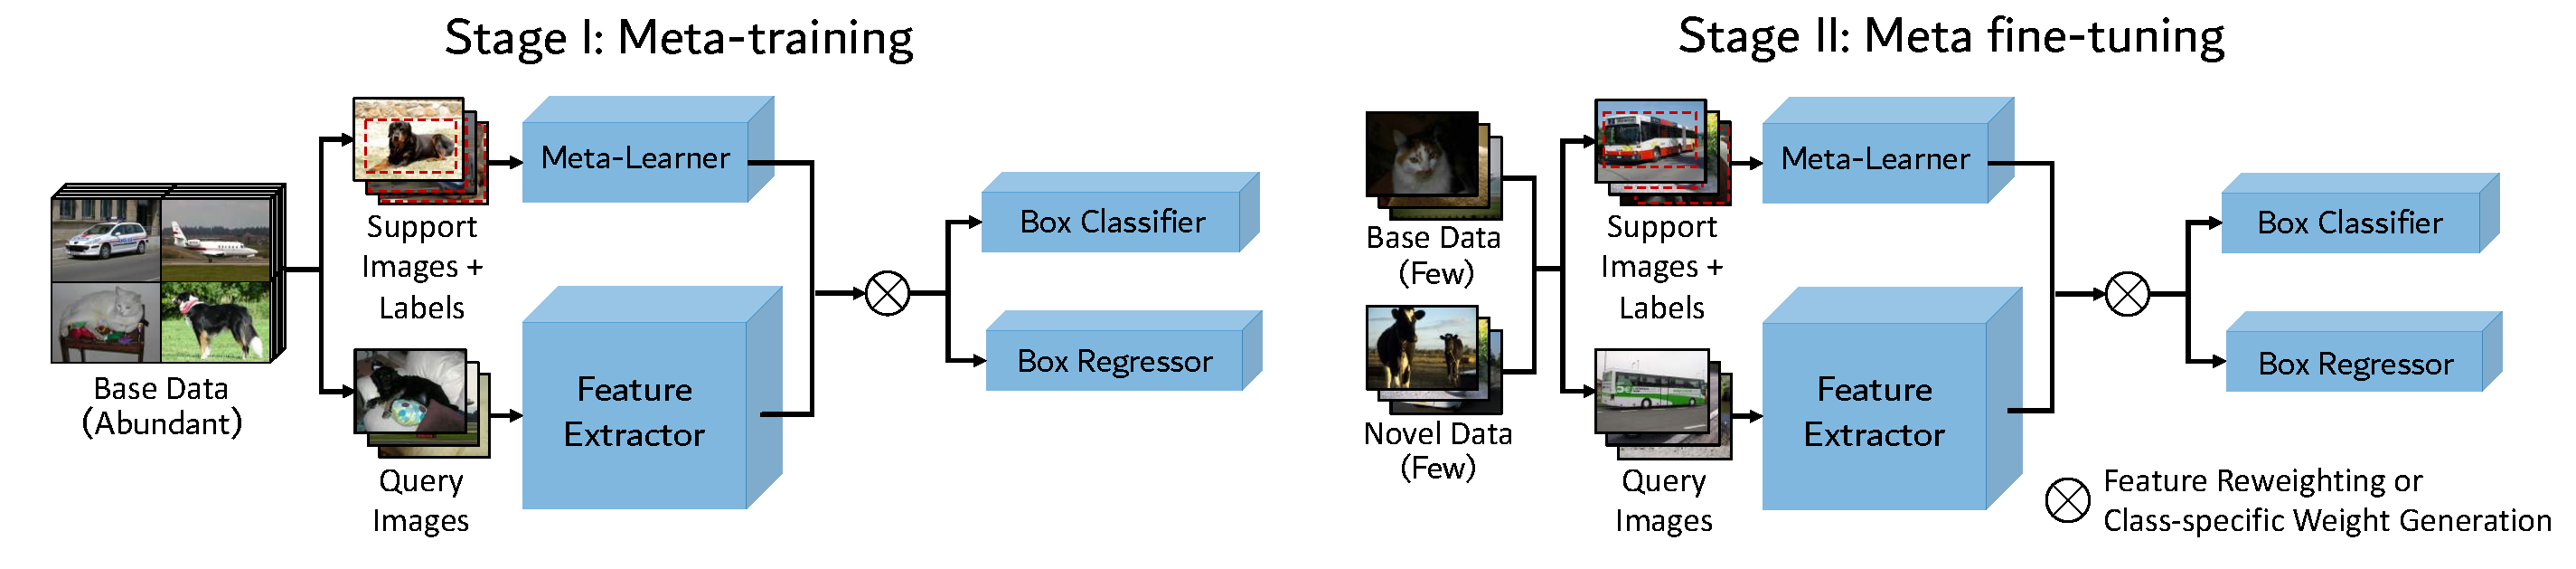
\includegraphics[width=\linewidth]{figs/TFA_fig2.pdf}
    \vspace{-8mm}
    \caption{Meta-learning based few-shot object detectors. A meta-learner is used to help the model generalize to novel classes. A two-stage training approach is adopted.}
    \label{fig:meta_arch}
\end{figure*}

\minisection{Cosine similarity for box classifier.} The design of the classifier is based on the cosine similarity function, inspired by ~\citet{gidaris2018dynamic,qi2018low}.
The weight matrix of the box classifier is $W\in\mathbb{R}^{d\times c}$, where $w_c\in\mathbb{R}^d$ is the per-class weight vector. The output of $\mathcal{C}$ is scaled similarity scores $S$
\begin{equation}
    s_{i,j} = \frac{\alpha \mathcal{F}(x)_i^\top w_j}{\|\mathcal{F}(x)_i\| \|w_j\|},
    \label{eq:classifier} 
\end{equation}
where $s_{i,j}$ is the similarity calculated between the $i$-th proposed object and the weight vector of class $j$. $\alpha$ is a scaling factor. We use a fixed $\alpha$ of 20 and use instance-level feature normalization in our experiments to help diminish the variance.

\subsection{Compared Meta-learning with Fine-tuning}
\label{sec:meta}
Both the meta-learning method (See Figure~\ref{fig:meta_arch}) and our method are composed of two stages. However, since our fine-tuning method only fine-tunes the last layer of the network, our method is much more memory efficient than the meta-learning method.
